% !TEX root = ../my-thesis.tex
%
\chapter{Related Work}
\label{sec:related}

\section{Prior related work: }

The topic of this thesis was built upon the work of many of colleagues at IPP. The work done by D. Böckenhoff et al. in their 2018 paper \cite{Böckenhoff_2018} laid down the fundemental research that motivated this thesis. They set out to use artificial neural networks to reconstruct $I_B$, the coil current from the $B$-coils (seen in the following diagram \ref{fig:3}), the from heat load in the experiment. Since they used the $\iota$-scan data from the prior OP1.1 experimental campaign, which used a limiter, their work is applied to a very different data set. The limiter that was used in W7X for the OP1.1 campaign is a piece of graphite designed to interface with the plasma to prevent it from interacting with the wall, potentially damaging the wall surface. A divetor plays a similar role to a limiter but in addition to acting as a plasma interface to protect the wall there is a subdivertor space that helps compress neutral gas which helps with the pumping process. Because of this additional function the form of the divertor used in the OP1.2 data is quite different (see figure \ref{fig:limiter-divertor}). As an additional note: the OP2 experiment will include a water cooled divetor, which can impact the heat load recorded by the thermal cameras.

\begin{figure}[!htb]
    \centering
    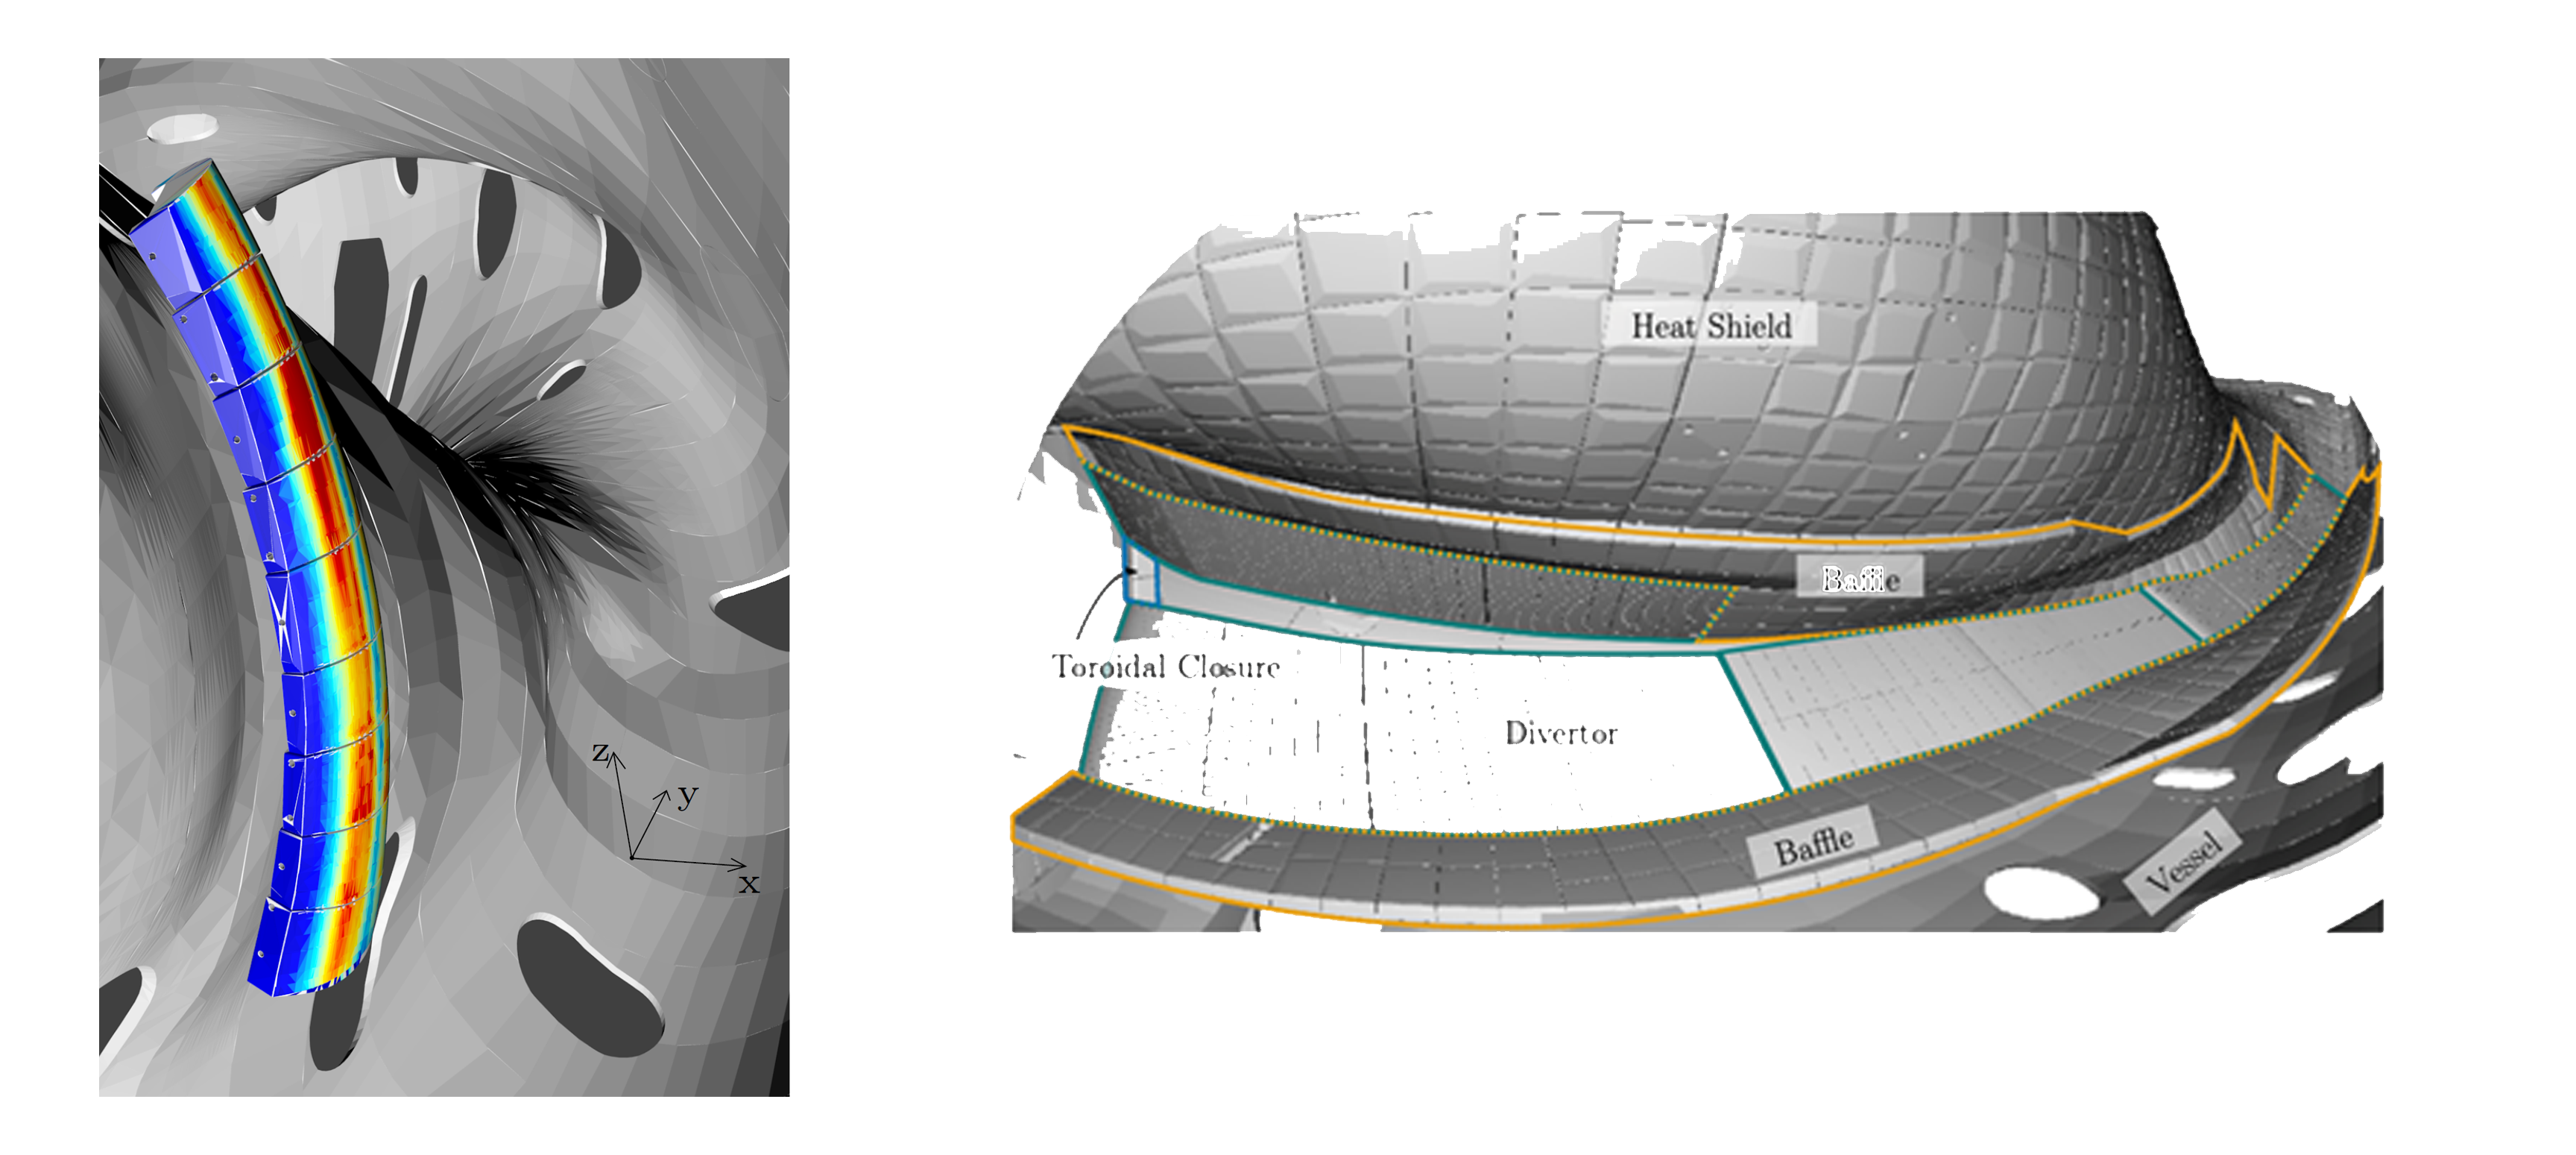
\includegraphics[width = \textwidth]{images/limiter-divetor.png}
    \caption{Left: Three-dimensional representation of heat flux on the surface of a limiter in W7X. Taken from \cite{Böckenhoff_2018} Right: } \label{fig:limiter-divetor}
\end{figure}

In the paper from D. Böckenhoff et al., data was limited to 6 values of $I_B$ taken from actual experimental data. While they were able to reconstruct $I_B$ using only the real world data with an $rmse$ (root mean squared error) of 0.047 for the test set results when using interpolated and extrapolated data. However, the performance on extrapolated data was notably worse. To improve these results they went a step further and used synthetic data using simulated $\iota$-scan data. A new version of the network was trained explicitly on the synthetic data and the validation set was entirely synthetic as well. The resulting network worked well, however, there was an observed systematic underestimation of $I_B$ of $-0.026 \pm 0.001$.

The best results came from using the neural network pretrained on synthetic data and trained on the real data set after. The combination yielded the best results, with an $rmse$ of 0.013 and better performance on extrapolated results overall.

In the 2018 paper "Neural network performance enhancement for limited nuclear fusion experiment observations supported by simulations" from M. Blatzheim et al. \cite{Blatzheim_2018}, the authors refined the methods used in the 2018 paper to improve the neural network performance. This paper also works with the data from the OP1.1 and worked with a mix of measured and simulated inputs and outputs.

In this paper they compared several neural network architectures, a fully connected feed-forward neural network with 3 layers of 64 notes each, a neural network composed of a series four 5x5, eight 3x3, and 16 more 3x3 convolutional filters followed by two fully connected layers, and a shallow network composed of an inception module, followed by pooling, a 1x1 convolutional layer, and two fully connected layers.

Different partitions of the input image were used. The input resolutions were $9x5$, $18x8$, $72x15$, $144x30$. Also, three different input parameterization of the partitions were tested: $(\mu, \sigma)$, $(\mu, \delta)$, and $\rho$. The $\mu$ and $\sigma$ parameterization is the standard deviation of the heat load, $\mu$ is the mean of the heat load, and $\delta$ is the difference between the maximum and minimum heat load values. The $\rho$ parameterization is the relative heat load. Increasing the number of inputs also resulted in a higher number of network parameters to accommodate the increased input size.

\begin{figure}[!htb]
    \centering
    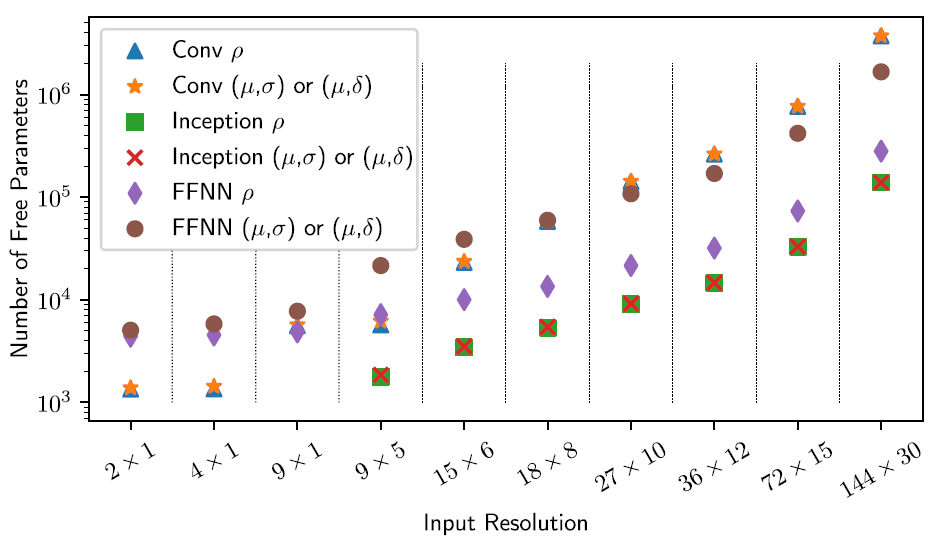
\includegraphics[width = \textwidth]{images/daniel-input-parameters.png}
    \caption{The free parameters of the NN based on the input resolution, parameterization, and architecture.} \label{fig:daniel-input-parameters}
\end{figure}

Solid results were found with the $9x5$ and $36x12$ resolutions using a convolutional NN and mixed real world and simulated data using the $\rho$ parameterization, achieving an $rmse$ of 0.008. The inception model showed improved performance for higher resolution inputs and could be useful for data like that from the OP1.2 campaign.

The results from M. Blatzheim et al. were used as a baseline for the final paper in the series, "Neural Network Regression Approaches to Reconstruct Properties of Magnetic Configuration from Wendelstein 7-X Modeled Heat Load Patterns" \cite{Blatzheim_2019}. The authors used the results from the previous papers to improve the neural network performance but unlike the prior papers which were using data from the OP 1.1 campaign which used a limiter, this paper looks at heat load data from the divertor that was added for the OP 1.2 campaign. Since this thesis is also using data from the OP 1.2 campaign, the results from this paper helped to inform the methods used in this thesis.

In this paper the authors used two targets for training.

% \begin{equation}
% 	\begin{align*}
% 		 & \Delta R=c_1 \cdot \Delta \tilde{R}\left(I_{\mathrm{A}}, I_{\mathrm{B}}\right)+c_2 \cdot \Delta R_{\mathrm{S}}                   \\
% 		 & t=c_3 \cdot \tilde{t}\left(I_{\mathrm{A}}, I_{\mathrm{B}}\right)+c_4 \cdot t_{I_{\mathrm{tor}}}\left(I_{\mathrm{tor}}\right)+t_0
% 	\end{align*}
% \end{equation}

One of the issues with the dataset used in the 2019 paper is that the reconstruction problem is more complex compared to the limiter configurations used in the 2018 papers. Despite the complexity, the papers authors produced several neural architectures that performed well both in $rmes$ and with a 5-fold cross validation. Good results were achieved with a convolutional neural network but the network was shallow compared to some of the deeper networks which tested better.